
\chapter{多面角和正多面体}

\section{多面角}

有公共端点并且不在同一平面内的几条射线，以及相邻两条射线间的平面部分所组成的图形，叫做\textbf{多面角}.

相邻的两面墙和地板所成的角，棱锥中各条侧棱所在的射线及侧面所在的两条射线间的平面部分所组成的图形，都是多面角.

如图3.1、3.2、3.3都是多面角.


\noindent
\begin{minipage}{.32\textwidth}
    \centering
\begin{tikzpicture}
\tkzDefPoints{0/0/S, 2/0/C, 0/2/A, -1/-1/B}
\tkzDrawSegments(B,S A,S S,C)
\tkzLabelPoints[above](A)
\tkzLabelPoints[left](B)
\tkzLabelPoints[right](C)
\tkzLabelPoints[above right](S)
 \draw[decorate, decoration={random steps, segment length=3pt, amplitude=2pt}] 
        (A)to [bend left](C) (A)to [bend right](B)  (B)to [bend right](C);

\end{tikzpicture}
\captionof{figure}{}
\end{minipage}\hfill
\begin{minipage}{.32\textwidth}
    \centering
    \begin{tikzpicture}
\tkzDefPoints{0/2/S, -1.2/.5/A', -.7/0/B', .5/0/C', 1.3/.7/D', 0/1/E'}

\foreach \x in {A,B,C,D} 
{\tkzDefPointWith[linear, K=1.3](S,\x')
\tkzGetPoint{\x}}
\tkzDefPointWith[linear, K=2.3](S,E')
\tkzGetPoint{E}
\tkzDrawSegments(S,A S,B S,C S,D A',B' B',C' C',D')
\tkzDrawSegments[dashed](S,E A',E' E',D')
\tkzLabelPoints[below](A,B,C,D,E)
\tkzLabelPoints[above](S)

\end{tikzpicture}
\captionof{figure}{}
\end{minipage}\hfill
\begin{minipage}{.32\textwidth}
    \centering
    \begin{tikzpicture}
\tkzDefPoints{0/2/S, -1.2/.5/A', -.7/0/B', .05/.4/C', 1/.4/D', 0.2/1/E'}

\foreach \x in {A,B,C,D} 
{\tkzDefPointWith[linear, K=1.3](S,\x')
\tkzGetPoint{\x}}
\tkzDefPointWith[linear, K=2.3](S,E')
\tkzGetPoint{E}
\tkzDrawSegments(S,A S,B S,C S,D A',B' B',C' C',D')
\tkzDrawSegments[dashed](S,E A',E' E',D')
\tkzLabelPoints[below](A,B,C,D,E)
\tkzLabelPoints[above](S)

    
\end{tikzpicture}
\captionof{figure}{}
\end{minipage}


组成多面角的射线，如图中的$SA, SB,\ldots$叫做多面角的棱. 多面角的棱的公共点，如图中的$S$点叫做多面角的顶
点；相邻两棱间的平面部分叫做多面角的面；相邻两棱组成的角$\angle ASB,  \angle BSC,\ldots$叫做多面角的面角；多面角中相邻两个面所组成的二面角如 $E-SA-B,  A-SB-C,\ldots$叫做多面角的二面角.

从上述定义易知，一个多面角的棱数、面数、面角数、二面角数是相等的.

多面角最少应有三个面。多面角依照它的面数分别叫做三面角、四面角、五面角、…….

把一个多面角的任何一个面伸展成平面时，如果其他各面都在这个平面的同侧，这样的多面角叫做凸多面角. 图3.1、 3.2中的多面角都是凸多面角，图3.3中的多面角不是凸多面角.

对于一个凸多面角，如果用一个平面截它的各个面和棱，得到的多边形一定是凸多边形.

多面角可用表示它的顶点和棱的字母来表示，如图3.1中的多面角记作多面角$S-ABC$，图3.2、图3.3中的多面角分别记作多面角$S-ABCDE$、$S-ABCDE$. 有时也可以用表示顶点的一个字母来表示多面角. 记作多面角$S$.

我们在本章只研究凸多面角。以后讲到的多面角都是指凸多面角.

凸多面角中，最简单的是三面角. 三个面角都是直角的三面角叫做直三面角。例如屋角，桌角，箱子的一角都给我们以直三面角的形象，

直三面角$O-xyz$的一般画法如图3.4，图中$Ox$、$Oy$、$Oz$是三面角的棱，$M$、$N$、$P$是面，点$O$是三面角的顶点.

\begin{example}
    求证：直三面角的各个二面角都是直二面角.

已知：直三面角$O-xyz$（图 3.4）.

求证：二面角$P-Ox-M$、  $M-Oy-N$、  $N-Oz-x$ 都是直二面角.
\begin{figure}[htp]
    \centering
\begin{tikzpicture}
\tkzDefPoints{0/0/O, 2/0/y, 0/2/z, -1/-1/x}
\tkzDrawSegments(O,x O,y O,z)
\tkzLabelPoints[above](z)
\tkzLabelPoints[left](x)
\tkzLabelPoints[right](y)
\tkzLabelPoints[below](O)
 \draw[decorate, decoration={random steps, segment length=3pt, amplitude=2pt}] 
        (x)to [bend right](y) (y)to [bend right](z)  (x)to [bend left](z);
\node at (.45,-.5){$M$};
\node at (.7,1){$N$};
\node at (-.5,.7){$P$};
\end{tikzpicture}
    \caption{}
\end{figure}
\end{example}

\begin{proof}
$\because \quad O-xyz$是直三面角，

$\therefore\quad \angle xOy=\angle yOz
=\angle zOx={\rm Rt}\angle$,
$Oz\perp Ox,\quad Oy\perp Ox$.

$\therefore\quad  \angle yOz$ 是二面角$P-Ox-M$ 的平面角.

$\because\quad \angle yOz=\mathrm{Rt}\angle$, 

$\therefore\quad$ 二面角$P-Ox-M$ 是直二面角.

同理， $M-Oy-N$、$N-Oz-P$ 也是直二面角.
\end{proof}

\subsection*{3.1 练习}
\begin{enumerate}
    \item 二面角为什么不是多面角？多面角和棱锥有什么区别？
    \item 
用一个平面截直三面角的三个面，得一截面是三角形，求证这三角形的垂心，是这三面角的顶点在这平面内的射影.
    \item 
求证：三个二面角都是直二面角的三面角是直三面角.
    \item 
一个三面角的两个面角相等，求证这两个面角所对的二面角也相等.
\end{enumerate}


\section{多面角的性质}

像多边形可以看作由若干个三角形组成的一样，任何一
个多面角，可以看作是由若干个三面角组成的. 例如四面
角，可以过一组相对的棱作平面将它分成两个三面角. 这个事实说明，三面角是研究多面角的基础.

\begin{thm}
{三面角的性质定理} 三面角的任意一个面角小于其他两个面角之和.
\end{thm}


已知：三面角$S-ABC$（图3.5）,

求证： $\angle ASB+\angle BSC>\angle ASC$.

\begin{figure}[htp]
    \centering
\begin{tikzpicture}
\tkzDefPoints{0/0/A', 4/0/C', 1/-1.3/B', 1.5/2/S, 1.5/-.5/D'}

\foreach \x/\y in {A/1.5,B/1.3,C/1.3} 
{
\tkzDefPointWith[linear, K=\y](S,\x')
\tkzGetPoint{\x}
\tkzLabelPoints[below](\x)
\tkzDrawSegments(S,\x)
}
\tkzDrawSegments(A',B' B',C')
\tkzDrawSegments[dashed](A',C' S,D')
\tkzLabelPoints[above](S)
\tkzLabelPoints[right](D',B')
\end{tikzpicture}
    \caption{}
\end{figure}

\begin{proof}
当$\angle ASC\le \angle ASB$ 时，显然有
\[
\angle ASC<\angle ASB+\angle BSC\]

现在设$\angle ASC>\angle ASB$，在面$ABC$内作线段$SD'$，使$\angle ASD' =\angle ASB$. 在$SB$上截取$SB' =SD'$. 过$D'$任意作一直线$A' C'$, 交$SA$于$A'$, 交$SC$于$ C' $, 连结 $A' B' $, $ B' C' $.
则$\triangle A' SB' \cong\triangle A' SD'$,

$\therefore\quad A' B' =A' D'$.

在$\triangle A' B' C'$中， $A' B' +B' C' >A' C' $，而
\[
A' C' =A' D' +D' C' =A' B' +D' C' 
\]

$\therefore\quad B' C' >D' C'$.

在$\triangle B' SC'$  和 $\triangle D' SC'$  中，
\[SB' =SD' ,\quad SC' =SC' ,\quad B' C' >C' D'\]

$\therefore\quad \angle B' SC' >\angle C' SD' $,

$\therefore\quad \angle B' SC' +\angle A' SB' >\angle C' SD' +\angle A' SD' $.

即 $\angle BSC+\angle ASB>\angle CSA$.
\end{proof}

\begin{thm}
{推论} 三面角的任何一个面角大于其他两个面角的差.
\end{thm}

\begin{thm}
{多面角的性质定理} 凸多面角所有面角的和小于 $360^{\circ}$.
\end{thm}

已知：凸$n$面角$S-ABC\cdots E$（图3.6）.

\begin{figure}[htp]
    \centering
\begin{tikzpicture}
\tkzDefPoints{0/2.5/S, -1.2/.5/A', -.7/0/B', .5/0/C', 1.3/.7/D', 0/.8/E'}

\foreach \x/\y in {A/1.5,B/1.5,C/1.5,D/1.5,E/1.8} 
{
\tkzDefPointWith[linear, K=\y](S,\x')
\tkzGetPoint{\x}
\tkzLabelPoints[below](\x)
}

\tkzDrawSegments(S,A S,B S,C S,D A',B' B',C' C',D')
\tkzDrawSegments[dashed](S,E A',E' E',D')

\tkzLabelPoints[above](S)
\tkzLabelPoints[left](A')
\tkzLabelPoints[right](D',C')
\tkzLabelPoints[above right](E')
\tkzLabelPoints[below left](B')
\end{tikzpicture}
    \caption{}
\end{figure}

求证：$\angle ASB+\angle BSC+ \cdots +\angle ESA<360^{\circ}$.

\begin{proof}
用平面截已知多面角的所有的面和棱，得到凸多边形
$A' B' C' \cdots E'$. 则以$A'$、 $B'$、  $C'$……$E'$为顶点的各三面角有下列关系式：
\[\begin{split}
   \angle E' A' B' &<\angle SA' E' +\angle SA' B'\\ 
\angle A' B' C' &<\angle SB' A' +\angle SB' C' \\
\cdots&\cdots\\
\angle D' E' A' &<\angle SE' D' +\angle SE' A' 
\end{split}\]

令$\Sigma=\angle ASB+\angle BSC+\cdots +\angle ESA$. 将上面各不等式两边分别相加，左边是凸多边形$A' B'\cdots E'$所有内角的和，右边是$n$个三角形的内角和与$\Sigma$的差. 因此，
\[
2(n-2)\cdot 90^{\circ}<n\cdot 180^{\circ}-\Sigma\]

$\therefore\quad \Sigma <n\cdot 180^{\circ}-2n\cdot 90^{\circ}+360^{\circ}=360^{\circ}$.

\begin{figure}[htp]
    \centering
\begin{tikzpicture}[scale=.9]
\begin{scope}
\def\x{30}
\draw(\x-72:1.8)node[below]{$A$}--(\x:2)node[right]{$B$}--(\x+72:2)node[above]{$S$}--(\x+144:2)node[left]{$D$}--(\x+216:1.8)node[below]{$A$};
\draw(\x-72:1.8)--(\x+72:2)--(\x+216:1.8);
\draw(-.3,.9)node[below]{$C$}--(\x+72:2);
\draw[dashed](\x+144:2)--(-.3,.9)--(\x:2);
\node at (3,0){$\implies$};
\end{scope}
\begin{scope}[xshift=6cm]
\tkzDefPoint(45:2.2){A}
\tkzDefPoint(0,0){S}
\tkzDefPoint(45+90:2){B}
\tkzDefPoint(45+170:2.1){C}
\tkzDefPoint(-100:2){D}
\tkzDefPoint(-50:2.2){A'}
\foreach \x in {A,B,C,D,A'} 
{
    \draw(S)--(\x);
}
\draw(A)--(B)--(C)--(D)--(A');
\tkzLabelPoints[left](B,C)
\tkzLabelPoints[right](A,S)
\tkzLabelPoints[below](D)
\node at (-50:2.2)[right]{$A$};

\end{scope}
\end{tikzpicture}
    \caption{}
\end{figure}
\end{proof}

这个性质表明，如果沿凸多面角的一条棱剪开，把它展开铺在平面上，那么它不能铺满一个周角，而是缺少一部分（图3.7）。

\section*{习题一}
\begin{enumerate}
    \item 下列各面角能否构成三面角？
\begin{multicols}{2}
\begin{enumerate}[(1)]
    \item $100^{\circ},\quad 90^{\circ},\quad 150^{\circ}$;
    \item $82^{\circ},\quad 56^{\circ},\quad 26^{\circ}$;
    \item $130^{\circ},\quad 85^{\circ},\quad 36^{\circ}$;
    \item $75^{\circ},\quad 45^{\circ},\quad 90^{\circ}$.
\end{enumerate}

\end{multicols}
    \item 下列各组面角能否构成四面角？
\begin{multicols}{2}
\begin{enumerate}[(1)]
      \item $45^{\circ},\quad 60^{\circ},\quad 120^{\circ},\quad 95^{\circ}$;
    \item $50^{\circ},\quad 70^{\circ},\quad 100^{\circ},\quad 150^{\circ}$;
    \item $75^{\circ},\quad 105^{\circ},\quad 120^{\circ},\quad 60^{\circ}$;
    \item $150^{\circ},\quad 30^{\circ},\quad 70^{\circ},\quad 40^{\circ}$.
\end{enumerate}

\end{multicols}
    \item 在三面角中，如果有两个二面角是直二面角，那么它们所对的两个面角都是$\underline{\qquad\qquad}$角.

    \item 直三面角$O-XYZ$内有一点$P$, $OP$在三面角三个面上的射影分别是$a$、$b$、$c$，则 $OP=\underline{\qquad\qquad}$

    \item 在三面角$S-ABC$中， $\angle BSC=90^{\circ}$,  $\angle ASB=  \angle ASC=60^{\circ}$
\begin{enumerate}[(1)]
\item 设$SA=SB=SC$，求证：经过三点$A$、$B$、$C$的平面垂直于$\angle BSC$ 所在的平面；
\item 求证：$SA$与$\angle BSC$ 所在的平面成$45^{\circ}$的角.
\end{enumerate}
    
    \item 求证在三面角中，较大二面角所对的面角也较大.

    \item 求证：空间四边形每相邻两边所成的四个角的和小于$ 360^{\circ}$.

    \item 求证：多面角的任何一个面角不能等于 $180^{\circ}$.

    \item 从平面外一点向平面引两条斜线，如果它们和平面所成的角分别为$64^{\circ}$ 和$ 23^{\circ}$, 求这两条斜线夹角的范围.
\end{enumerate}



\section{欧拉定理}


\subsection{简单多面体}

表面通过连续变形，可变为球面的多面体叫做简单多面体.

这里说的连续变形，可理解为橡皮变形，设想图形在橡皮膜上，当橡皮膜变形时，有的地方伸长，有的地方压缩，但不破裂，不折叠. 这样橡皮膜上的图形也跟着改变，这种图形的变化过程就是连续变形. 例如正六面体可连续变形成为一个球（图3.8），所以正六面体是一简单多面体. 同理，棱柱、棱锥、棱台、圆锥等凸多面体都是简单多面体.

\begin{figure}[htp]
    \centering
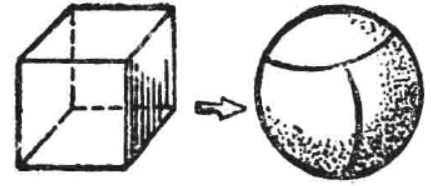
\includegraphics[scale=.4]{fig/3-8.png}
    \caption{}
\end{figure}

多面体中，也有不是简单多面体的. 例如长方体穿透一个洞所得的多面体，连续变形后就不能变为一个球面而只能变成一个环面（图3.9）.
\begin{figure}[htp]
    \centering
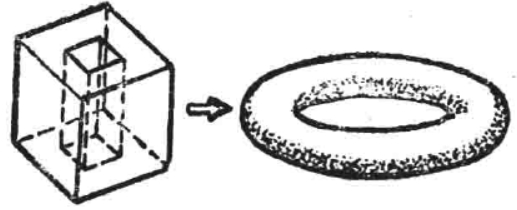
\includegraphics[scale=.4]{fig/3-9.png}
    \caption{}
\end{figure}

如果我们用$V$表示简单多面体的顶点数，$E$表示这多面体的棱数，$F$表示这多面体的面数. 请同学们数一下下面这些简单多面体的$V$、$E$、$F$各是多少？它们之间有什么关系吗？

\begin{figure}[htp]
    \centering
\begin{tikzpicture}[scale=.9]
\begin{scope}
\tkzDefPoints[]{0/0/A, 3/0/B, 1.3/-1/C, 0.5/2/A', 2.5/2/B', 1.3/1.3/C'}
\tkzDrawPolygon[](A,C,B,B',A')
\tkzDrawSegments[](C,C' C',A' C',B')
\tkzDrawSegments[dashed](A,B)
\node at (1.5,-1.5){I};
\end{scope}

\begin{scope}[xshift=4cm]
\tkzDefPoints[]{0/0/A, 2/0/B, 1.5/-.5/C, 0/2.2/A'}
\tkzDefPointsBy[translation=from A to A'](B,C){B',C'}
\tkzDrawPolygon[](A,C,B,B',A')
\tkzDrawSegments[](C,C' C',A' C',B')
\tkzDrawSegments[dashed](A,B)
\node at (1,-1.5){II};
\end{scope}

\begin{scope}[xshift=7cm]
\tkzDefPoints[]{0/0/A, 1.75/-.2/B, 1/-.7/C, 1/2/S}
\tkzDrawPolygon[](S,A,C,B)
\tkzDrawSegments[](S,C)
\tkzDrawSegments[dashed](A,B)
\node at (1,-1.5){III};
\end{scope}

\begin{scope}[xshift=10cm]
\tkzDefPoints[]{0/-.5/A, 1/-.5/B, -.25/0/E, 1.5/0/C, .6/.3/D, .6/2/S}
\tkzDrawPolygon[](S,E,A,B,C)
\tkzDrawSegments[](S,A S,B)
\tkzDrawSegments[dashed](S,D C,D D,E)
\node at (.5,-1.5){IV};
\end{scope}

\begin{scope}[yshift=-4cm]
\tkzDefPoints{0/0/A, 3/0/A', -.5/1/B, 3.25/1/B', .5/2/C, 2.7/2/C'}
\tkzDrawPolygon[](A,B,C)
\tkzDrawPolygon[](A',B',C')
\tkzDrawSegments[](A',A C,C')
\tkzDrawSegments[dashed](B,B')
\node at (1.5,-.5){V};
\end{scope}

\begin{scope}[yshift=-5.5cm, xshift=4cm]
\tkzDefPoints{0/0/A, 2.25/0/B, 3/.75/C, 0/2.25/A'}
\tkzDefPointsBy[translation=from B to C](A){D}
\tkzDefPointsBy[translation=from A to A'](B,C,D){B',C',D'}
\tkzDrawPolygon[](A,B,C,C',D',A')
\tkzDrawSegments[](B',B C,C' B',A' B',C')
\tkzDrawSegments[dashed](D,A D,D' D,C)
\node at (1.5,-.5){VI};
\end{scope}

\begin{scope}[yshift=-5cm, xshift=8cm]
\tkzDefPoints{0/0/A, 2.25/0/B, 3/.75/C, 0/2.25/A'}
\tkzDefPointsBy[translation=from B to C](A){D}
\tkzDefPointsBy[translation=from A to A'](B,C,D){B',C',D'}
\tkzDefPointWith[linear, K=.7](B,B') \tkzGetPoint{mid1}
\tkzDefPointWith[linear, K=.3](B',C') \tkzGetPoint{mid2}
\tkzDefPointWith[linear, K=.7](A',B') \tkzGetPoint{mid3}
\tkzDrawPolygon[](mid1,mid2,mid3)
\tkzDrawSegments[](A,B B,C C,C' A,A' C',D' D',A' B,mid1 A',mid3 C',mid2)
\tkzDrawSegments[dashed](D,A D,D' D,C)
\node at (1.5,-.5){VII};

\end{scope}

\begin{scope}[yshift=-7cm]
\tkzDefPoints[]{-.25/0/A, .8/-.6/B, 2.5/-.2/C, 1.25/1.25/S1, 1/-1.5/S2}
\tkzDefPointsBy[translation=from B to A](C){D}
\tkzDrawPolygon[](S1,A,S2,C)
\tkzDrawSegments[](A,B B,C B,S1 B,S2)
\tkzDrawSegments[dashed](D,S1 D,S2 C,D D,A)
\node at (1,-2){VIII};
\end{scope}

\begin{scope}[yshift=-9cm, xshift=6cm]
\tkzDefPoints{0/0/A, 2.25/0/B, 3/.75/C, 0/2.25/A', 2/3.5/S}
\tkzDefPointsBy[translation=from B to C](A){D}
\tkzDefPointsBy[translation=from A to A'](B,C,D){B',C',D'}

\tkzDrawSegments[](B,B' C,C' A,A' A,B B,C A',B' B',C' S,A' S,B' S,C' S,D' A',D')
\tkzDrawSegments[dashed](D,A D,D' D,C C',D')
\node at (1.5,-.5){IX};

\end{scope}
\end{tikzpicture}
    \caption{}
\end{figure}


\begin{enumerate}[(1)]
    \item 是否面的数目$F$都随顶点的数目增大而增大？
    \item 是否棱的数目$E$都随顶点的数目增大而增大？
    \item $V$、$E$、$F$之间有什么等量关系吗？
\end{enumerate}

为了便于分析概括，列表如下.

\begin{center}
    \begin{tabular}{ccccc}
    \hline
    编号&	多面体名称&	顶点数($V$)&	面数($F$)&	棱数($E$)\\
    \hline
I	&立方体&	8&	6	&12\\
II&	三棱柱&	6&	5&	9\\
III&	三棱锥&	4&	4	&6\\
IV	&五棱锥&	6&	6	&10\\
V&	三棱台	&6&	5&	9\\
VI&	楔体&	6&	5&	9\\
VII&	截角立方体&	10&	7	&15\\
VIII	&八面体&	6&	8	&12\\
IX	&“塔顶”体&	9&	9&	16\\
\hline
\end{tabular}
\end{center}


我们发现，面的数目$F$并不随顶点数目的增大而增大.如八面体和立方体的顶点数是由6增大到8，而面数却由8减小到6.

棱的数目$E$也并不是随顶点数目的增大而增大的，如“塔顶”体和截角立方体的顶点数由9增大到10，而棱数却由16
减少到15.

为了发现规律，我们试按一种数目，例如棱数的增大为顺序，重新排列上表如下：

\begin{center}
  \begin{tabular}{ccccc}
    \hline
编号&	多面体&	顶点数($V$)&	面数($F$)&	棱数($E$)\\
    \hline
III	&三棱锥&	4&	4	&6\\
II	&三棱柱&	6&	5	&9\\
V	&三棱台&	6&	5&	9\\
VI	&楔体 &	6 &	5	&9\\
IV	&五棱锥&	6&	6	&10\\
VIII	&八面体&	6&	8	&12\\
I	&立方体&	8&	6	&12\\
VII	&截角立方体&	10&	7&	15\\
IX	&“塔顶”体&	9	&9	&16\\
\hline
\end{tabular}  
\end{center}


我们发现，当棱数增大时，面数和棱数总的来说也在增大，但面数和顶点数都有减小的，进一步我们发现，凡是面
数减小时，顶点数却在增加；顶点数减小时，面数在增加.

容易发现，对其中任何一个多面体，它的顶点数$V$、棱数$E$和面数$F$有下述关系：
\[
F+V=E+2\]

\subsection{欧拉定理}

上面我们发现的关系式对任何简单多面体都是成立的，这就是著名的欧拉定理.
\begin{thm}
{定理} 简单多面体的顶点数$V$、棱数$E$、面数$F$，有下面的关系
\[
V+F-E=2\]
\end{thm}


下面我们进行证明.

\noindent
\begin{minipage}{0.65\textwidth}
  \CTEXindent 设多面体的各棱具有弹性可以伸长和缩短，我们把多面体的一个面剪掉，剩余的部分和原多面体相比，只是少了一个面，而它的棱数和顶点数都未改变，设想把“剪口”多边形拉到最大，把其余各多边形都“压在”这个多边形内，使它们都在同一平面内. 由于原来是多面体时，过每个顶点的
棱数至少有三条，又棱长可以伸缩，所以可使在同一平面内的各多边形的每个内角都小于$180^{\circ}$, 从而使各多边形都是凸多边形（如图3.11）.
\end{minipage}
\hfill
\begin{minipage}{0.3\textwidth}
  \centering
\begin{tikzpicture}[scale=.8]
\tkzDefPoints{0/1/A, 2/1/B, 3.5/2.8/C, 1.8/5/D, -.5/4.8/E, -1.5/3/F}
\tkzDrawPolygon[](A,B,C,D,E,F)
\tkzDefPoints{0.2/4/M1, 1.5/3.9/M2, 0.5/3/M3}
\tkzDrawPolygon[](M1,M2,M3)
\tkzDefPoints{0.5/2/N1, 1.75/2/N2, 1.4/2.8/N3}
\tkzDrawPolygon[](N1,N2,N3)
\tkzDrawSegments(A,N1 B,N2 C,N2 M1,E  M2,D M3,N1 N3,M2)

\end{tikzpicture}
    \captionof{figure}{}
\end{minipage}


设“最大”多边形有$n$条边，则有$n$个顶点，原多面体的顶点
数是$V$，那么被包围在这个多边形内的顶点数是$(V-n)$. 因而，被围的各个小多边形的所有内角和是：
\[
(V-n)\cdot  360^{\circ}+(n-2)\cdot  180^{\circ}\]
再加上剪掉的一个多边形的内角和就是
\[
(V-n)\cdot  360^{\circ}+(n-2)\cdot  180^{\circ}+(n-2)\cdot  180^{\circ}
=(V-2)\cdot  360^{\circ}\tag{1}\]

因为凸多边形的内角和只与边数有关，而与多边形的形状和大小无关，所以上述的内角和$(V-2)\cdot  360^{\circ}$ 就是原多面体的所有面角的总和.

我们再从另一个角度来计算一下具有$F$个面，$E$个棱的多面体所有面角的和应是多少？

设多面体的$F$个面（多边形）中，边数分别是$n_{1},n_{2},\ldots,n_F$. 我们分别计算各面（多边形）的内角和.

\begin{center}
\begin{tabular}{ccc}
\hline
多边形编号&	边数	&内角和\\
\hline
1	&$n_{1}$	&$\left(n_{1}-2\right)\cdot  180^{\circ}$\\
2	&$n_{2}$	&$\left(n_{2}-2\right)\cdot  180^{\circ}$\\
……	&……&	……\\
$F$	&$n_{F}$&	$\left(n_{F}-2\right)\cdot  180^{\circ}$\\
\hline
\end{tabular}
\end{center}

$\therefore\quad$ 所有面角的总和是：
\[
\left(n_{1}+n_{2}+\cdots+n_{F}\right)\cdot  180^{\circ}-2F\cdot  180^{\circ}\]

$\because\quad$ 每条棱同属于两个面，即每一棱都是两个多边形的公共边. 

$\therefore\quad n_{1}+n_{2}+\cdots+n_{F}=2E$.

$\therefore\quad \left(n_{1}+n_{2}+\cdots+n_{F}\right)\cdot  180^{\circ}-2F\cdot  180^{\circ}
=2(E-F)\cdot  180^{\circ}\qquad (2)$

由(1)、(2)得
\[
(V-2)\cdot  360^{\circ}=2(E-F)\cdot  180^{\circ}\]

$\therefore\quad V-2=E-F$, 即$V+F-E=2$.

由于任何简单多面体，都可以通过连续变形变成凸多面
体. 所以上述证明过程中，虽然用到多面体的各面是凸多边形，但是欧拉定理不仅对凸多面体成立，而且对任何简单多面体都是成立的.

欧拉定理表明，一个简单多面体，经过连续变形后，尽管它的形状可以变化万千，但有一个数始终不变，即顶点数$+$面数$-$棱数，它总是2，所以2这个数又叫做简单多面体连续变形下的不变数.

\section{正多面体}

每个面都是有同数边的正多边形，在每个顶点都是有同数棱的凸多面体，叫做正多面体.

例如，正方体的所有面都是有4个边的正四边形，在每个顶点都有三条棱，而且是凸多面体，所以正方体是一种正多面体.

\begin{thm}
{问1} 使两个全等的正三棱锥的底面相重合，所形成的六面体是正多面体吗？
\end{thm}

\begin{thm}
{问2} 把问1中的正三棱锥换为正四面体呢？
\end{thm}


正多边形有无限多种，如正三角形、正方形、正五边形、正六边形、……正多面体呢？下面来研究这个问题.

设正多面体每个面都是正$n$边形，在每个顶点的棱数都是$m$（从而每个顶点都是$m$面角的顶点）.

由于凸$m$面角的面角都是正$n$边形的内角，正$n$边形的内角即凸$m$面角的每个面角等于
\[
\frac{2(n-2)\cdot  90^{\circ}}{n}\]

所以凸$m$面角所有面角之和是
\[
\frac{2m(n-2)\cdot  90^{\circ}}{n}\]

根据凸多面角性质
\[
\frac{2m(n-2)\cdot  90^{\circ}}{n}<360^{\circ}\]
化简得
$m(n-2)<2n$,
即
\[
m<\frac{2n}{n-2}\qquad \text{（$m$,$n$都是不小于3的整数）}\]
解这个不等式，
\begin{itemize}
    \item 当$n=3$时，$m<6$，得$m=3,4,5$;

    \item 当$n=4$时，$m<4$，得$m=3$;

    \item 当$n=5$时，$m<\frac{10}{3}$，得$m=3$.
\end{itemize}

因为$n>5$ 时， $m<3$不合题意，故$n$不能大于5. 
所以一个正多面体，它的面的边数$n$，顶点数$m$应该满足上述条件，即正多面体只能有五种. 我们可以做出这种正多面体. 它们是：用正三角形做面的正四面体、正八面体、正二十面体，在它们每个顶点的棱数分别是3、4、5；用正方形做面的正六面体，在它每个顶点的棱数是3；用正五边形做面的正十二面体，在它每个顶点的棱数也是3，这五种正多面体的直观图如图3.12所示.
\begin{figure}[htp]
    \centering
\begin{tikzpicture}
\begin{scope}
\tkzDefPoints{0/.8/A, 2.5/.8/B, 1.8/0/C, 1.5/2.5/S}
\tkzDrawPolygon[](S,A,C,B)
\tkzDrawSegments[dashed](A,B)
\tkzDrawSegments(S,C)
\end{scope}
\begin{scope}[xshift=3cm]
\tkzDefPoints{0/0/A, 2/0/B, 2.75/0.75/C, 0/2/A'}
\tkzDefPointsBy[translation=from B to C](A){D}
\tkzDefPointsBy[translation=from A to A'](B,C,D){B',C',D'}
\tkzDrawPolygon[](A,B,C,C',D',A')
\tkzDrawSegments[dashed](D,A C,D D,D')
\tkzDrawSegments(B,B' B',A' B',C')

\end{scope}
\begin{scope}[xshift=8cm]
\tkzDefPoints{-1/1/A, -.2/.75/B, 1.5/1.2/C}
\tkzDefPointsBy[translation=from B to C](A){D}
\tkzDefPoints{0.3/2.5/S1, 0.2/-.25/S2}
\tkzDrawPolygon[](S1,A,S2,C)
\tkzDrawSegments[dashed](D,S1 D,S2 D,A D,C)
\tkzDrawSegments[](B,A B,C B,S1 B,S2)



\end{scope}
\begin{scope}[yshift=-2cm, xshift=3cm]
\foreach \x in {0,1,2,3,4}
{
    \tkzDefPoint(-90+\x*72:1){A_\x}
    \tkzDefPoint(90+\x*72:1.25){B_\x}
}
\tkzDrawPolygon[dashed](A_0,A_1,A_2,A_3,A_4)
\tkzDrawPolygon[](B_0,B_1,B_2,B_3,B_4)

\foreach \x in {0,1,2,...,9}
{
    \tkzDefPoint(90+\x*36:1.65){C_\x}
}
\tkzDrawPolygon[](C_0,C_1,C_2,C_3,C_4,C_5,C_6,C_7,C_8,C_9)
\tkzDrawSegments[](B_0,C_0 B_1,C_2 B_2,C_4 B_3,C_6 B_4,C_8)
\tkzDrawSegments[dashed](A_0,C_5 A_1,C_7 A_2,C_9 A_3,C_1 A_4,C_3)
\end{scope}
\begin{scope}[yshift=-2cm, xshift=7cm]
\foreach \x in {0,1,2}
{
    \tkzDefPoint(90+\x*120:1){A_\x}
    \tkzDefPoint(-90+\x*120:1){B_\x}
}
\tkzDrawPolygon[dashed](A_0,A_1,A_2)
\tkzDrawPolygon[](B_0,B_1,B_2)

\foreach \x in {0,1,2,...,5}
{
    \tkzDefPoint(90+\x*60:1.65){C_\x}
}
\tkzDrawPolygon[](C_0,C_1,C_2,C_3,C_4,C_5)

\tkzDrawSegments[dashed](A_0,C_0 A_1,C_2 A_2,C_4)
\tkzDrawSegments[](B_0,C_3 B_1,C_5 B_2,C_1)
\tkzDrawSegments[dashed](A_0,C_1 A_0,C_5 A_1,C_1 A_1,C_3 A_2,C_5 A_2,C_3)
\tkzDrawSegments[](C_0,B_2 C_0,B_1 C_2,B_2 C_2,B_0 C_4,B_0 C_4,B_1)

\end{scope}
\end{tikzpicture}
    \caption{}
\end{figure}

正多面体的表面展开图如图3.13所示，据此可以作出这五种正多面体的模型.


\begin{figure}[htp]
    \centering
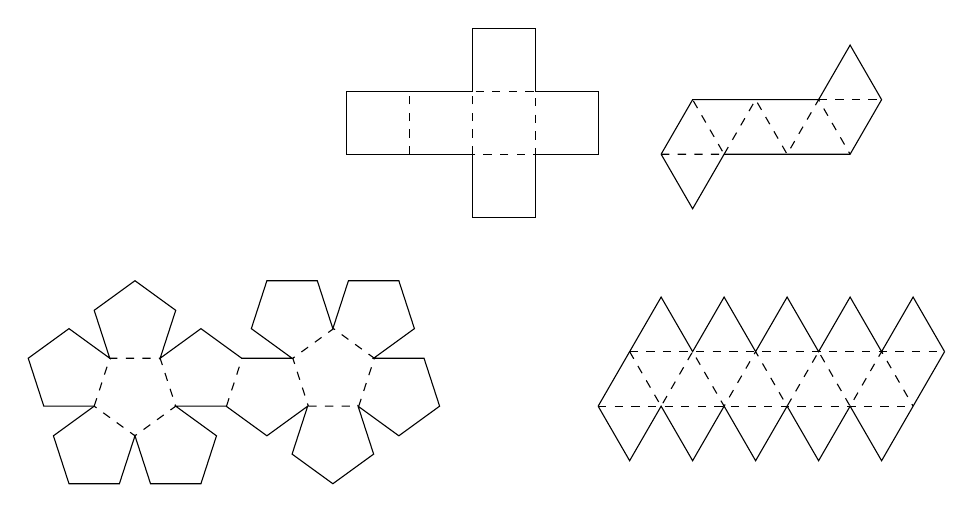
\begin{tikzpicture}[scale=.8]
\begin{scope}
\tkzDefPoints{0/0/A, 3/0/B, 1.5/2.6/C, 1.5/0/A'}
\tkzDefMidPoint(C,A) \tkzGetPoint{C'}
\tkzDefMidPoint(C,B) \tkzGetPoint{B'}
\tkzDrawPolygon[](A,B,C)
\tkzDrawPolygon[dashed](A',B',C')

\end{scope}
\begin{scope}[xshift=4cm, yshift=1cm]
\draw(0,0)--(2,0)--(2,-1)--(3,-1)--(3,0)--(4,0)--(4,1)--(3,1)--(3,2)--(2,2)--(2,1)--(0,1)--(0,0);
\draw[dashed](2,0)rectangle (3,1);
\draw[dashed](1,0)--(1,1);
\end{scope}
\begin{scope}[xshift=9cm, yshift=1cm]
\draw(0,0)--(60:1)--++(2,0)--++(60:1)--++(-60:1)--++(-120:1)--++(-2,0)--++(-120:1)--++(120:1);
\draw[dashed](0,0)--(1,0)--++(120:1);
\draw[dashed](1,0)--++(60:1)--++(-60:1)--++(60:1)--++(-60:1);
\draw[dashed](2.5,.866)--++(1,0);
\end{scope}
\begin{scope}[yshift=-3cm]
    \def\x{.8}
\draw(0,0)--(-144:\x)--++(-72:\x)--++(0:\x)--++(72:\x)--++(-72:\x)--++(0:\x)--++(72:\x)--++(144:\x)--++(0:\x);
\draw(0,0)--++(180:\x)--++(108:\x)--++(36:\x)--++(-36:\x)--++(108:\x)--++(36:\x)--++(-36:\x)--++(-108:\x)--++(36:\x)--++(-36:\x)--++(0:\x)--++(144:\x)--++(72:\x)--++(0:\x)--++(-72:\x)--++(72:\x)--++(0:\x)--++(-72:\x)--++(-144:\x)--++(0:\x)--++(-72:\x)--++(-144:\x)--++(144:\x)--++(-72:\x)--++(-144:\x)--++(144:\x)--++(72:\x)--++(-144:\x)--++(144:\x);

\draw[dashed](0,0)--++(72:\x)--++(0:\x)--++(-72:\x)--++(-144:\x)--++(144:\x);
\draw[dashed](2.1,0)--++(72:\x);

\draw[dashed](3.4,0)--++(0:\x)--++(72:\x)--++(144:\x)--++(-144:\x)--++(-72:\x);
\end{scope}
\begin{scope}[xshift=8cm, yshift=-3cm]
\draw(0,0)--++(-60:1)--++(60:1)--++(-60:1)--++(60:1)--++(-60:1)--++(60:1)--++(-60:1)--++(60:1)--++(-60:1)--++(60:2);
\draw(0,0)--++(60:2)--++(-60:1)--++(60:1)--++(-60:1)--++(60:1)--++(-60:1)--++(60:1)--++(-60:1)--++(60:1)--++(-60:1);
\draw[dashed](0,0)--(5,0);
\draw[dashed](0.5,.866)--++(5,0);
\draw[dashed](60:1)--++(-60:1)--++(60:1)--++(-60:1)--++(60:1)--++(-60:1)--++(60:1)--++(-60:1)--++(60:1)--++(-60:1);

\end{scope}
\end{tikzpicture}
    \caption{}
\end{figure}


显然，正多面体都是简单多面体，所以它们的顶点数$V$，面数$F$和棱数$E$都满足欧拉定理的关系式
$V+F-E=2$.

\begin{example}
    试求与棱长为$a$的正四面体所有的棱都相切的球的半径.
\end{example}

\begin{analyze}
    正四面体有六条棱，它们都相等，我们知道正方
体有六个面，它们都是正方形，因而它们的对角线相等，如图3.14，正方体的六个面中对角线$B_{1}D_{1}$, $D_{1}C$, $CB_{1}$, $AB_{1}$, $AD_{1}$,  $AC$恰好构成正四面体的六条棱，正方体的内切球在各面的切点与各对角线相切. 因而正方体的内切球就是与对应的面对角线构成的正面体各棱相切的球. 它的半径就是正方体棱长的一半.
\end{analyze}


因为正四面体棱长为$a$，所以以它的棱为面对角线的正方体的棱长是$\frac{\sqrt{2}}{2}a$. 这正方体内切球的半径
\[
r=\frac{1}{2}\cdot \frac{\sqrt{2}}{2}a=\frac{\sqrt{2}}{4}a
\]
这就是与正四面体所有的棱都相切的球的半径.

\noindent
\begin{minipage}{.45\textwidth}
\centering
\begin{tikzpicture}
\tkzDefPoints{0/0/A, 2/0/B, 2.5/.7/C, 0/2/A_1}
\tkzDefPointsBy[translation=from B to C](A){D}
\tkzDefPointsBy[translation=from A to A_1](B,C,D){B_1,C_1,D_1}

\tkzDrawPolygon[](A,B,C,C_1,D_1,A_1)
\tkzDrawSegments[](B,B_1 B_1,D_1 A,B_1 C,B_1 A_1,B_1 B_1,C_1)
\tkzDrawSegments[dashed](A,C A,D_1 C,D_1 C,D A,D D,D_1)
\tkzLabelPoints[left](A,A_1,D_1)
\tkzLabelPoints[right](B,B_1,C_1,C)
\tkzLabelPoints[below right](D)


\end{tikzpicture}
\captionof{figure}{}
\end{minipage}
\begin{minipage}{.45\textwidth}
    \centering
\begin{tikzpicture}[scale=1.1]
    \tkzDefPoints{0/0/A, 2/0/B, 1.5/.7/C, 0/2/A'}
\tkzDefPointsBy[translation=from B to C](A){D}
\tkzDefPointsBy[translation=from A to A'](B,C,D){B',C',D'}
\tkzDrawPolygon[](A,B,B',C',D',D)
\tkzDrawSegments[](A,A' A',B' A',D')
\tkzDrawSegments[dashed](B,C C,D C,C')
\tkzDefMidPoint(A,D') \tkzGetPoint{a}
\tkzDefMidPoint(A,B') \tkzGetPoint{f}
\tkzDefMidPoint(A',C') \tkzGetPoint{d}
\tkzDefMidPoint(C',D) \tkzGetPoint{e}
\tkzDefMidPoint(B,D) \tkzGetPoint{b}
\tkzDefMidPoint(B',C) \tkzGetPoint{c}

\tkzDrawSegments[dashed](a,d a,b a,e a,f c,d c,b c,e c,f d,e d,f b,e b,f)



\end{tikzpicture}
\captionof{figure}{}
\end{minipage}




\begin{example}
    设正方体的棱长为$a$，求以这个正方体各面的中心为顶点的正八面体的体积.
\end{example}



\begin{solution}
如图3.15，正八面体相对两顶点的距离就是正方体相对两面的距离，即为$a$, 

$\therefore\quad$ 正八面体的棱长是$\frac{\sqrt{2}}{2}a$,

$\therefore\quad V_{\text{正八面体}}=\frac{1}{3}\cdot \left(\frac{\sqrt{2}}{2}a\right)^{2}\cdot  a=\frac{1}{6}a^{3}$.
\end{solution}

\begin{example}
    求正八面 相相 邻两面所成的二面角的大小.
\end{example}

\begin{figure}[htp]
    \centering
\begin{tikzpicture}
\tkzDefPoints{0/0/O, 0/2/V, 0/-2/G, -2/-.1/A, 2/.1/C, -.5/-1/B}
\tkzDefPointsBy[translation=from B to A](C){D}
\tkzDrawPolygon[](A,G,C,V)
\tkzDrawSegments[](A,B B,C B,G)
\tkzDrawSegments[dashed](A,D C,D V,D V,G)
\tkzDefMidPoint(A,D) \tkzGetPoint{E}
\tkzDrawSegments[dashed](V,E E,O E,G)
\tkzLabelPoints[left](A,E)
\tkzLabelPoints[right](C,O)
\tkzLabelPoints[below](G,D)
\tkzLabelPoints[above](V,B)

\end{tikzpicture}
    \caption{}
\end{figure}


\begin{solution}
    设$VABCDG$是正八面体（图3.16）. 作$VE\perp AD$于$E$，连结$GE$，则 $\angle VEG$ 是八面体相邻两面的二面角的平面角. 设$VA=a$,  $O$是正八面体的中心，则
\[
VO=AO=\frac{\sqrt{2}}{2}a,\qquad VE=\frac{\sqrt{3}}{2}a,\]
\[
\angle VEO=\arcsin\frac{VO}{VE}=\arcsin\frac{\frac{\sqrt{2}}{2}a}{\frac{\sqrt{3}}{2}a}=\arcsin\frac{\sqrt{6}}{3}\]
\[
\cos\angle VEG=1-2\sin^{2}\angle VEO=1-2\left(\frac{\sqrt{6}}{3}\right)^{2}=-\frac{1}{3}\]

$\therefore\quad \angle VEG=\arccos\left(-\frac{1}{3}\right)$.

正八面体相邻两面的二面角的大小是$\arccos\left(-\frac{1}{3}\right)$.
\end{solution}



\section*{习题二}
\begin{enumerate}
    \item 棱长为$a$的正八面体的对角线长是$\underline{\qquad\qquad}$.

    \item 以正四面体的高和棱为一边分别作正方形，则这两个正方形面积的比是$\underline{\qquad\qquad}$.

    \item 正八面体的棱长为$a$，则它的两个相对面的距离是$\underline{\qquad\qquad}$.
 \item 正方体各面中心是一个正八面体的顶点，则这正方体和正八面体体积之比是$\underline{\qquad\qquad}$.
 \item 正$n\; (n=4,8,20)$面体的棱长为$a$，它们的表面积的共同公式是$\underline{\qquad\qquad}$.
 \item 
正20面体的棱长为$a$, 连结相对顶点的对角线长为$b$，则它的体积是$\underline{\qquad\qquad}$.
 \item 
求证：正四面体的二面角与正八面体的二面角互补。
 \item 
求证：平行于正四面体的相对棱的平面，截这个正四面体的截面是一个矩形。
 \item 
就下面平面图形找出$V$、$E$、$F$的关系式（其中，$V$是三角形，或四边形的顶点数，$E$是所有小多边形边数的和（每个边仅计算一次）, $F$是多边形的个数（重叠的不计）.

\begin{center}
\begin{tikzpicture}[scale=0.85]
\begin{scope}
\tkzDefPoints{0/0/A, 2/0/B, 3/1.5/C, .5/2/D}
\tkzDrawPolygon[](A,B,C,D)
\tkzDrawSegments[](A,C B,D)
\end{scope}
\begin{scope}[xshift=3cm]
\tkzDefPoints{0/0/A, 3/0/B, 1.3/1.8/C, 1.3/1/D, 1.1/0.5/E}
\tkzDrawPolygon[](A,B,C)
\tkzDrawPolygon[](D,E,B)
\tkzDrawSegments[](A,E C,D)


\end{scope}
\begin{scope}[xshift=8cm, yshift=0.5cm]
\foreach \x in {0,1,2}
{
    \tkzDefPoint(90+120*\x:.6){A_\x}
    \tkzDefPoint(90+120*\x:1.5){B_\x}
    \draw(A_\x)--(B_\x);
}
\tkzDrawPolygon[](A_0,A_1,A_2)
\tkzDrawPolygon[](B_0,B_1,B_2)

\end{scope}
\begin{scope}[xshift=10.5cm]
\tkzDefPoints{0/0/A, 2/0/B, 3/1/C, 2/3/D, 0.5/2.5/E, -.5/1.2/F, 1/1/G}
\tkzDrawPolygon[](A,B,C,D,E,F)
\foreach \x in {A,B,C,D,E,F}
{
    \draw(G)--(\x);
}
\end{scope}
\end{tikzpicture}
\captionof*{figure}{（第9题）}
\end{center}


\item 已知：凸多面体的各面都是四边形，求证：$F=V-2$.

\end{enumerate}

\section{本章小结}

\subsection{知识结构分析}



\begin{center}
\begin{tikzpicture}[>=stealth]
\node (A1)at(0,0){多面角};
\node (A2)at(3,0){凸多面角};
\node (A3)at(6,0){三面角};
\node (A4)at(9,0){直三面角};
\draw[->](A1)--(A2);
\draw[->](A2)--(A3);
\draw[->](A3)--(A4);
\node[draw] (A5) at (3,-1){多面角的性质};
\node[draw] (A6) at (6,-1){三面角的性质};
\draw[->](A2)--(A5);
\draw[->](A3)--(A6);

\node (B1)at(1,-2){简单多面体};
\node (B2)at(4,-2){凸多面体};
\node (B3)at(7,-2){正多面体};
\draw[->](B1)--(B2);
\draw[->](B2)--(B3);
\node[draw] (B4) at (1,-3){简单多面体的性质};
\node[draw] (B5) at (7,-3){正多面体的性质};
\draw[->](B1)--(B4);
\draw[->](B3)--(B5);
\end{tikzpicture}
\end{center}

\subsection{几点说明}

\subsection*{关于基本内容}
\begin{enumerate}[(1)]
    \item 本章的主要内容是在第一章讲完二面角的基础上，介绍了多面角的概念及其主要性质，在第二章研究多面体的基础上研究了正多面体. 并用连续变形（也叫做拓扑变形）的方法证明了关于简单多面体的欧拉定理.

    \item 对于多面角，研究了它的重要的一类——凸多面角. 研究了最简单的多面角——三面角的性质，并在此基础上研究了凸多面角的一个重要性质.

    \item 对简单凸多面体，利用连续变形证明了欧拉定理 ($V+F-E=2$). 对于凹多面体，只要属于简单体可以连续变形为凸多面体，从而欧拉定理对这样的多面体也适用. 总之，欧拉定理应用的范围是简单多面体（不论凸凹）
    \item 对于正多面体，应注意它的概念包括三点，少了任何一点都不是多面体，这三点是：第一，必须是凸多面体；第二，多面体的每个面都是边数相同的正多边形；第三，每个顶点引出的棱数必须相同.还介绍了正多面体有且只有五种.以正三角形为面的有三种：正四面体，正八面体，正二十面体；以正四边形为面的一种：正方体；以正五边形为面的一种：正十二面体。正方面体都是简单多面体，因而欧拉定理对正多面体都适用.
\end{enumerate}



\subsection*{关于思想方法}
\begin{enumerate}[(1)]
 
   \item 把空间问题转化为平面问题是解决空间问题的基本方法. 本章中三面角性质的证明，就是通过作角和线段，把两个面角大小的比较问题转化为平面几何中“已知两三角形两边对应相等，则第三边大的夹角大”这个命题来进行的. 欧拉定理的证明，更是把多面体的所有顶点都“压”到一个平面上，利用平面凸多边形的性质进行证明的.


三面角的性质：“三面角的任一面角小于其他两个面角之和”和“三角形中任一边小于其他两边之和”具有完全相同的“结构”，前者可以视为后者在空间问题的推广.

   \item 在证明欧拉定理时，是利用了连续变形：假设简单多面体的面是用橡胶薄膜做成的.——为什么会这么想呢？实际上，我们知道欧拉定理所揭示的规律，无非是简单多面体的顶点数，棱数和面数这三个数之间的一个关系. 而这三个数与棱的长短，多边形在保持边数不变时的形状都是无关的，让这些无关的量任意变动，就是设想的“连续变形”. 这确实给我们考虑问题提供了一个很好的方法模型.

   \item 正多面体都有一个对称中心，都有以对称中心为球心
   的内切球和外接球，切点都是“均匀”分布的. 由此可以由正方体直观图的各面的中心（共六个点）连结出正八面体的直观图.由正方体的直观图中六个面中的六条对角线连结而成为正四面体的直观图，从而提供了画正四面体和正八面体的直观图的较为简便的方法.

正多面的对称性是在研究正多面体时可以利用的一个很好的性质. 例如在求八面体相邻两个面所成二面角的大小时，就是利用了“对称性”使证明步骤大大简化.

\end{enumerate}


\section*{复习题三}
\begin{enumerate}

    \item 用下列多边形，可以组成几种多面角？为什么？
\begin{multicols}{2}
\begin{enumerate}[(1)]
   \item 正三角形；  \item 正方形；  \item 正五边形；  \item 正六边形.
\end{enumerate}
\end{multicols}
    \item 在三面角$S-ABC$中， $\angle ASB=\angle ASC=45^{\circ}$,  $\angle BSC= 60^{\circ}$, 求证： $\angle BSC$所对的二面角是直二面角.

    \item 试证一个多面角中，它的任何一个面角不能等于$180^{\circ}$.

    \item 在三面角$V-ABC$中， $\angle BVC=90^{\circ}$, $\angle AVB=\angle AVC  =60^{\circ}$, 求$VA$与平面$BVC$所成的角.

    \begin{center}
\begin{tikzpicture}
\tkzDefPoints{0/0/V, 1.5/.8/A', 1.5/-1/B', 2.5/.3/C'}
\foreach \x in {A,B,C}
{
    \tkzDefPointWith[linear, K=1.3](V,\x') \tkzGetPoint{\x}
    \draw(V)--(\x)node[right]{$\x$};
}
\draw(A')--(C')--(B');
\draw[dashed](A')--(B');
\node at (0,0)[left]{$V$};
\end{tikzpicture}
\captionof*{figure}{（第4题）}
\end{center}


    \item 直三面角的三个面被任意平面所截，求证：截得的三角形的重心是三面角的顶点在截面上的射影.

    \item 已知一个简单多面体的各个顶点都有三条棱. 求证： $V=2F-4$.

    \item 求证：如果简单多面体的所有面都是奇数边的多边形，那么面数是偶数。
\end{enumerate}




